	\section{Configuration of Arduino IDE}
	
	In this section we will be looking at how to connect the Arduino Portenta H7 with a PC/laptop in order to use the board. Then, we will be going through the first steps of installing the relevant packages to use the Arduino Portenta H7 board and then we will be implementing a basic example sketch from the Arduino IDE.
	
	\subsection{Step-wise Configuration}
	
	\begin{enumerate}
		
		\item Connect the Arduino Portenta H7 board to the computer via USB Type-C cable.
		\item Press the reset button twice on the board and the LED on the board starts blinking green as shown in the Figure \ref{fig:Arduino PortentaH7 Connected to a Laptop} indicating that it is ready.
		
		
		
		\item Install the packages in order to use the Arduino Portenta board. To do this search for Portenta in the boards and select \textbf{Arduino Mbed OS Portenta Boards} and click install as shown in Figure \ref{fig:Installation Arduino Mbed OS Portenta Board}. After the installation is done, we can start writing sketches in the IDE.
	\end{enumerate}	
			
	\begin{center}
		\label{fig:Installation Arduino Mbed OS Portenta Board}
		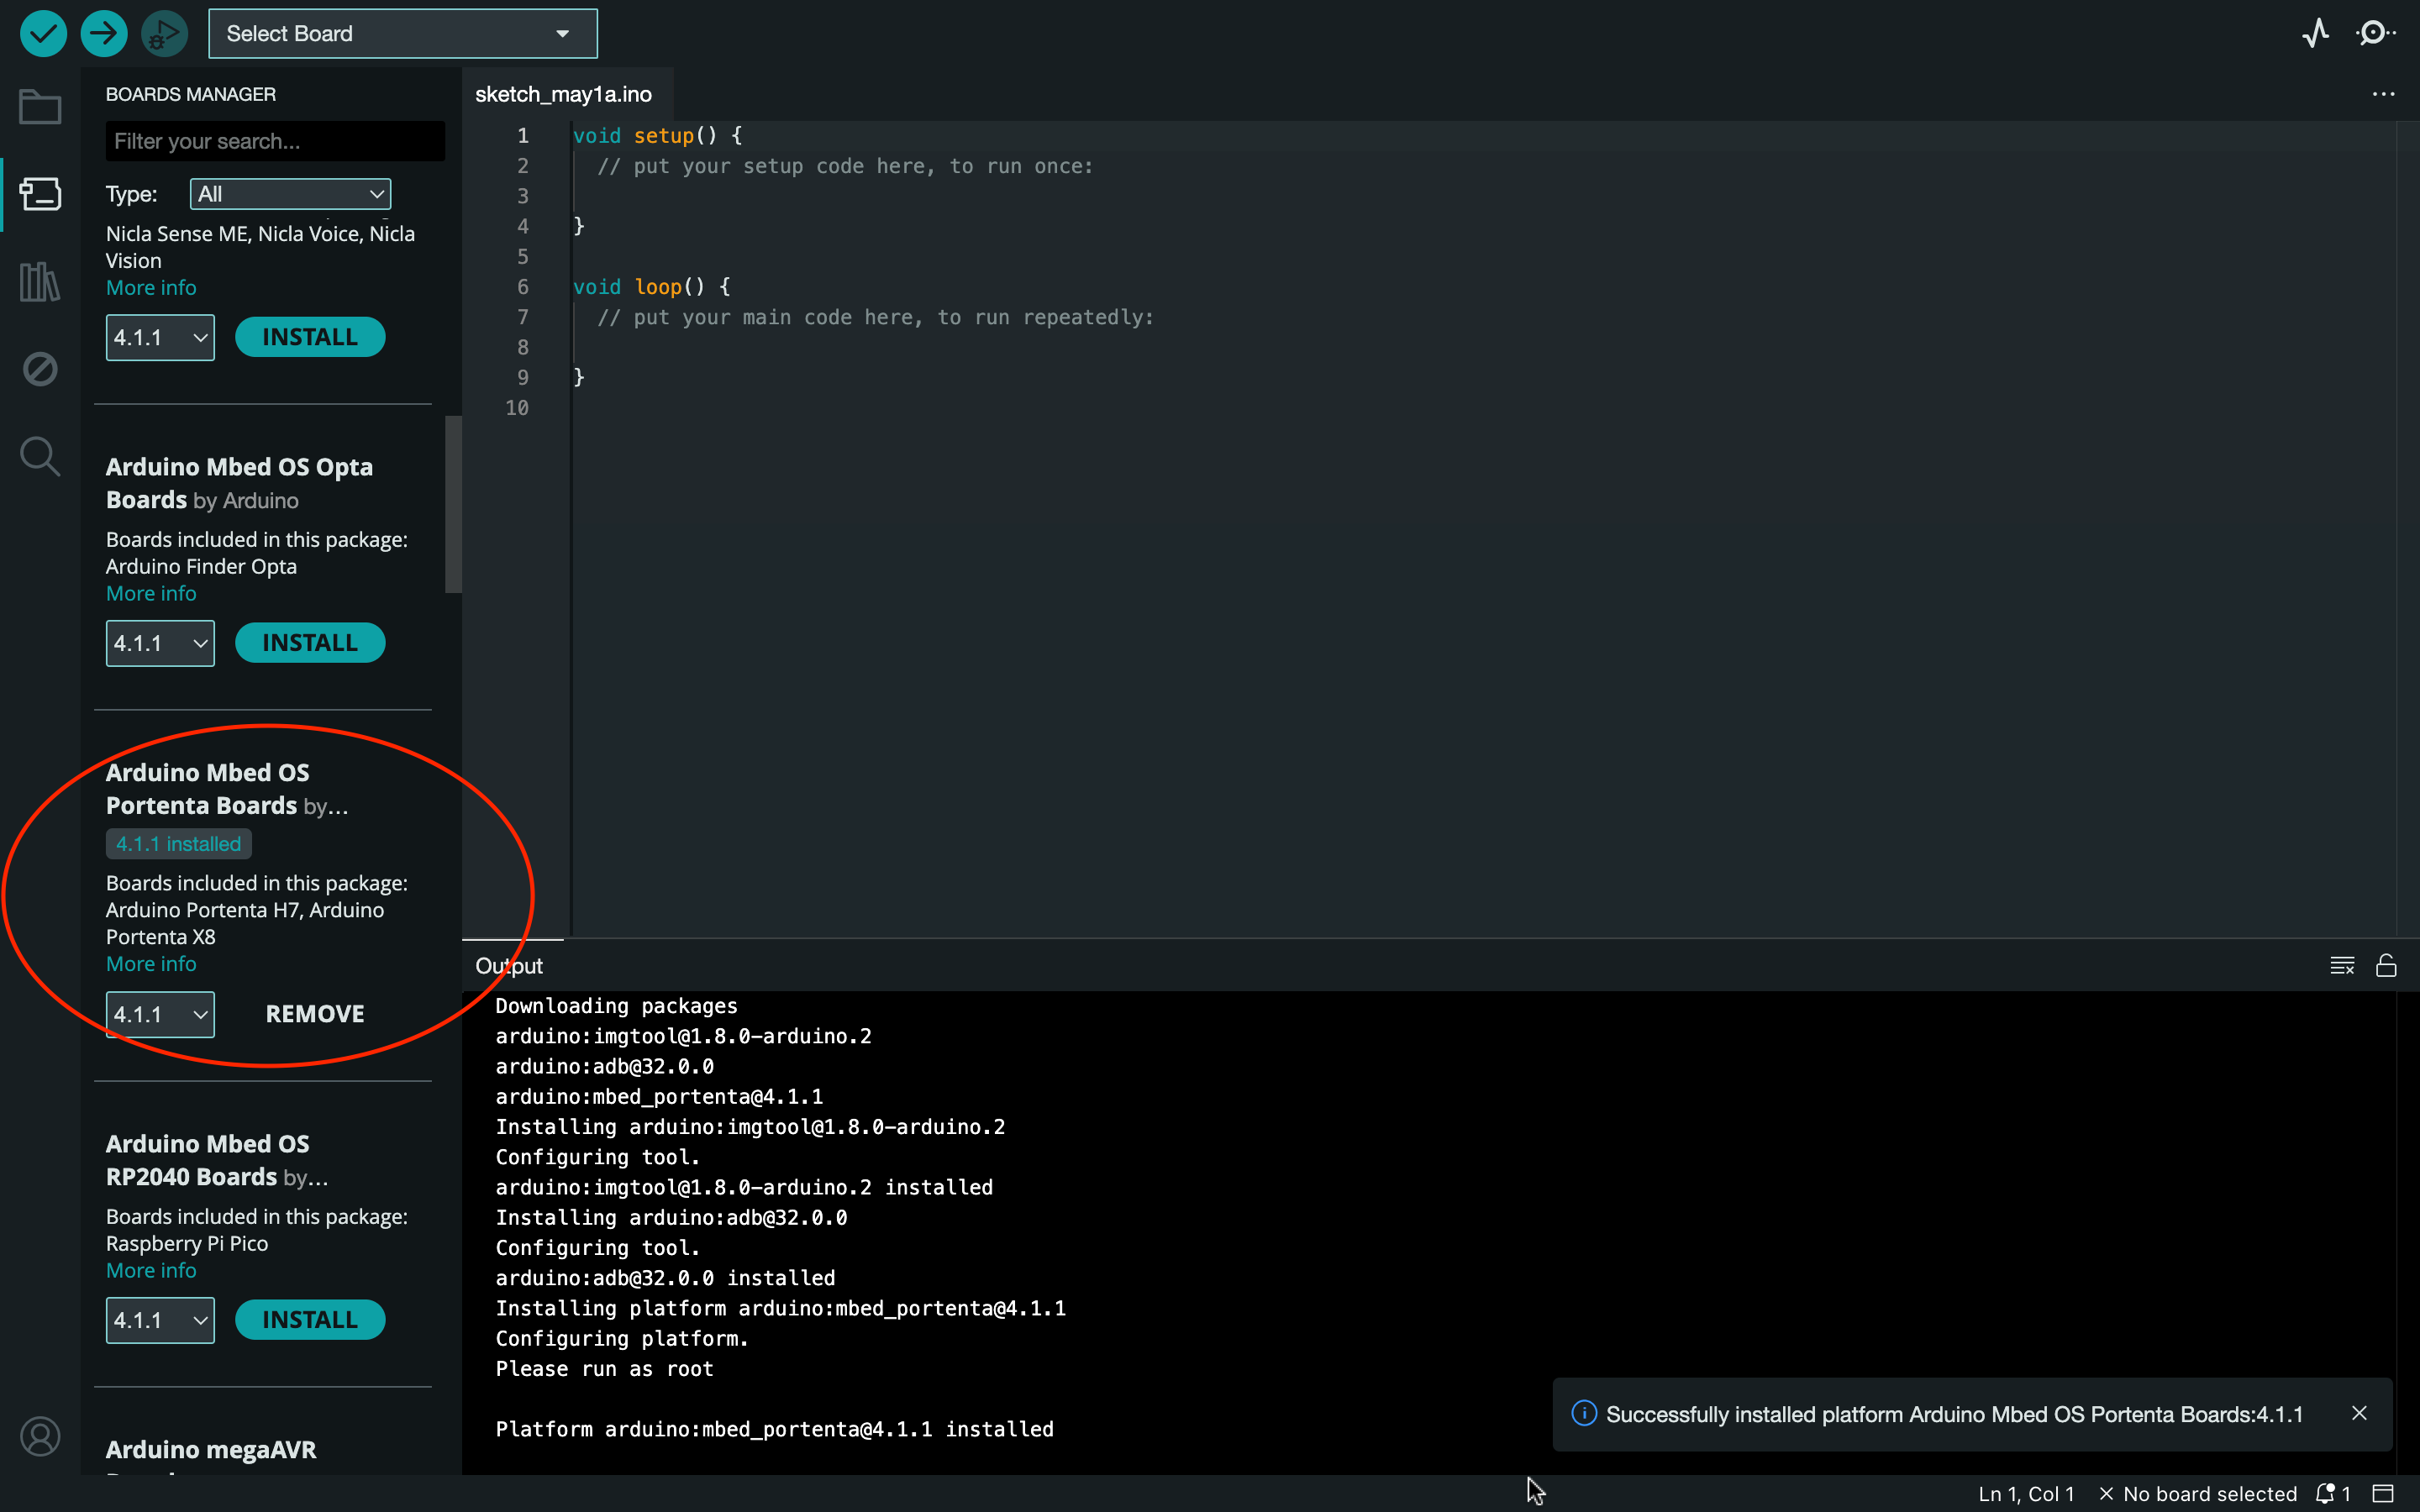
\includegraphics[width=0.7\linewidth]{images/ArduinoIDE/ArduinoMbedOSPortentaBoardsInstallation.png}
		\captionof{figure}{Installation Arduino Mbed OS Portenta Board}
	\end{center}
	
	
	\subsection{Example Blink Sketch}
	
	To upload the example sketch, go to File then click on examples and then click on 01.Basics and then select blink as shown in Figure \ref{fig:Example LED-Test}.
	
	\begin{center}
		\label{fig:Arduino PortentaH7 Connected to a Laptop}
		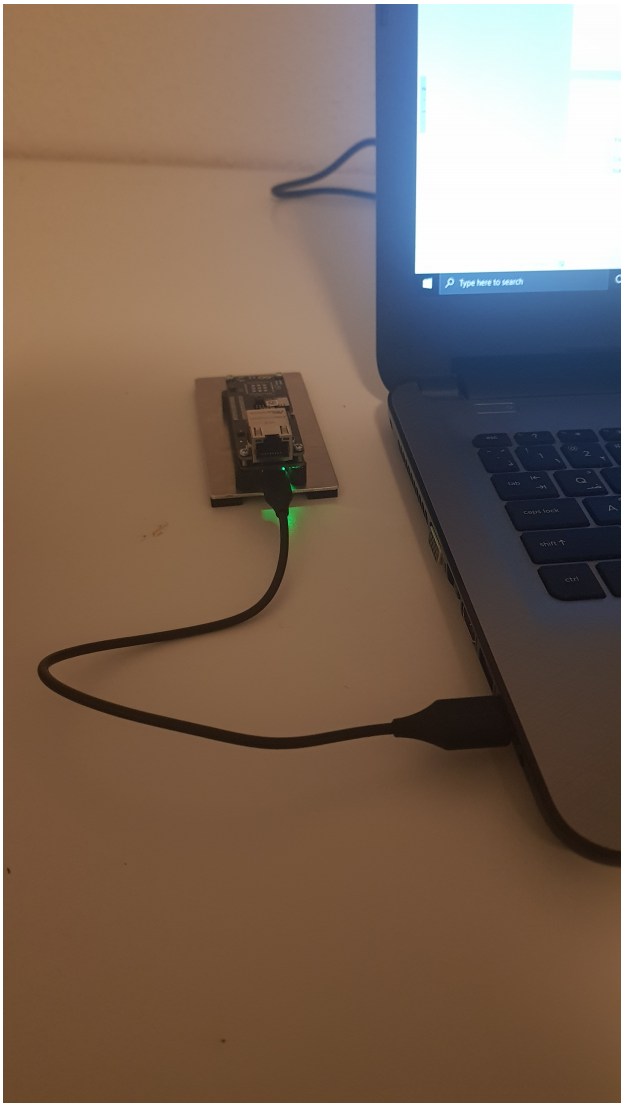
\includegraphics[width=0.7\linewidth]{images/ArduinoIDE/ArduinoPortentaH7Connectedtoalaptop.png}
		\captionof{figure}{Arduino PortentaH7 Connected to a Laptop}
	\end{center}
	
	\begin{center}
		\label{fig:Example LED-Test}
		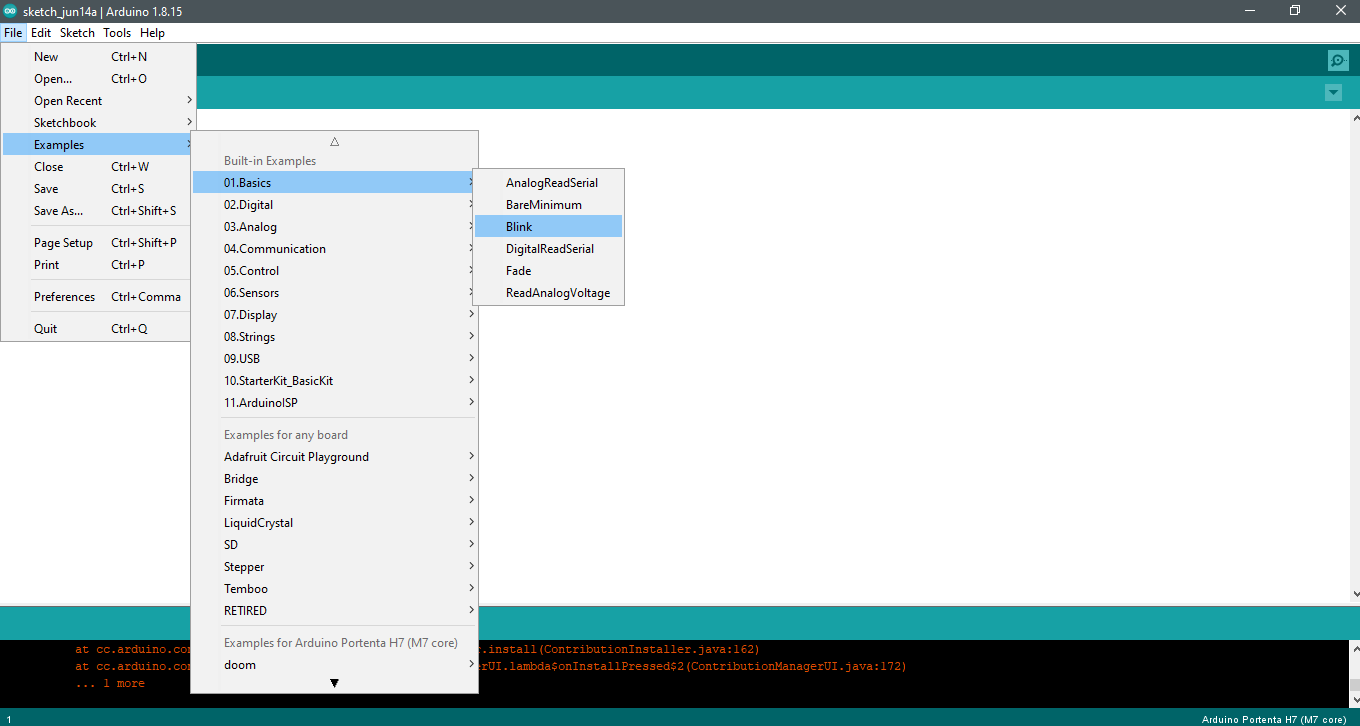
\includegraphics[width=0.7\linewidth]{images/ArduinoIDE/MenuBarOptions.png}
		\captionof{figure}{Example LED-Test}
	\end{center}
	
	
	In the program, we initialize LED\_BUILTIN as the output in the setup function. In the loop function we turn on the LED by using digitalWrite() function. Click on upload and wait for it to complete. After the upload is done, the green LED on the board starts blinking with a delay of 1000ms.The blink sketch appears on the screen as shown in Figure \ref{fig:Blink Sketch Compile}.
	
		\begin{center}
		\label{fig:Blink Sketch Compile}
		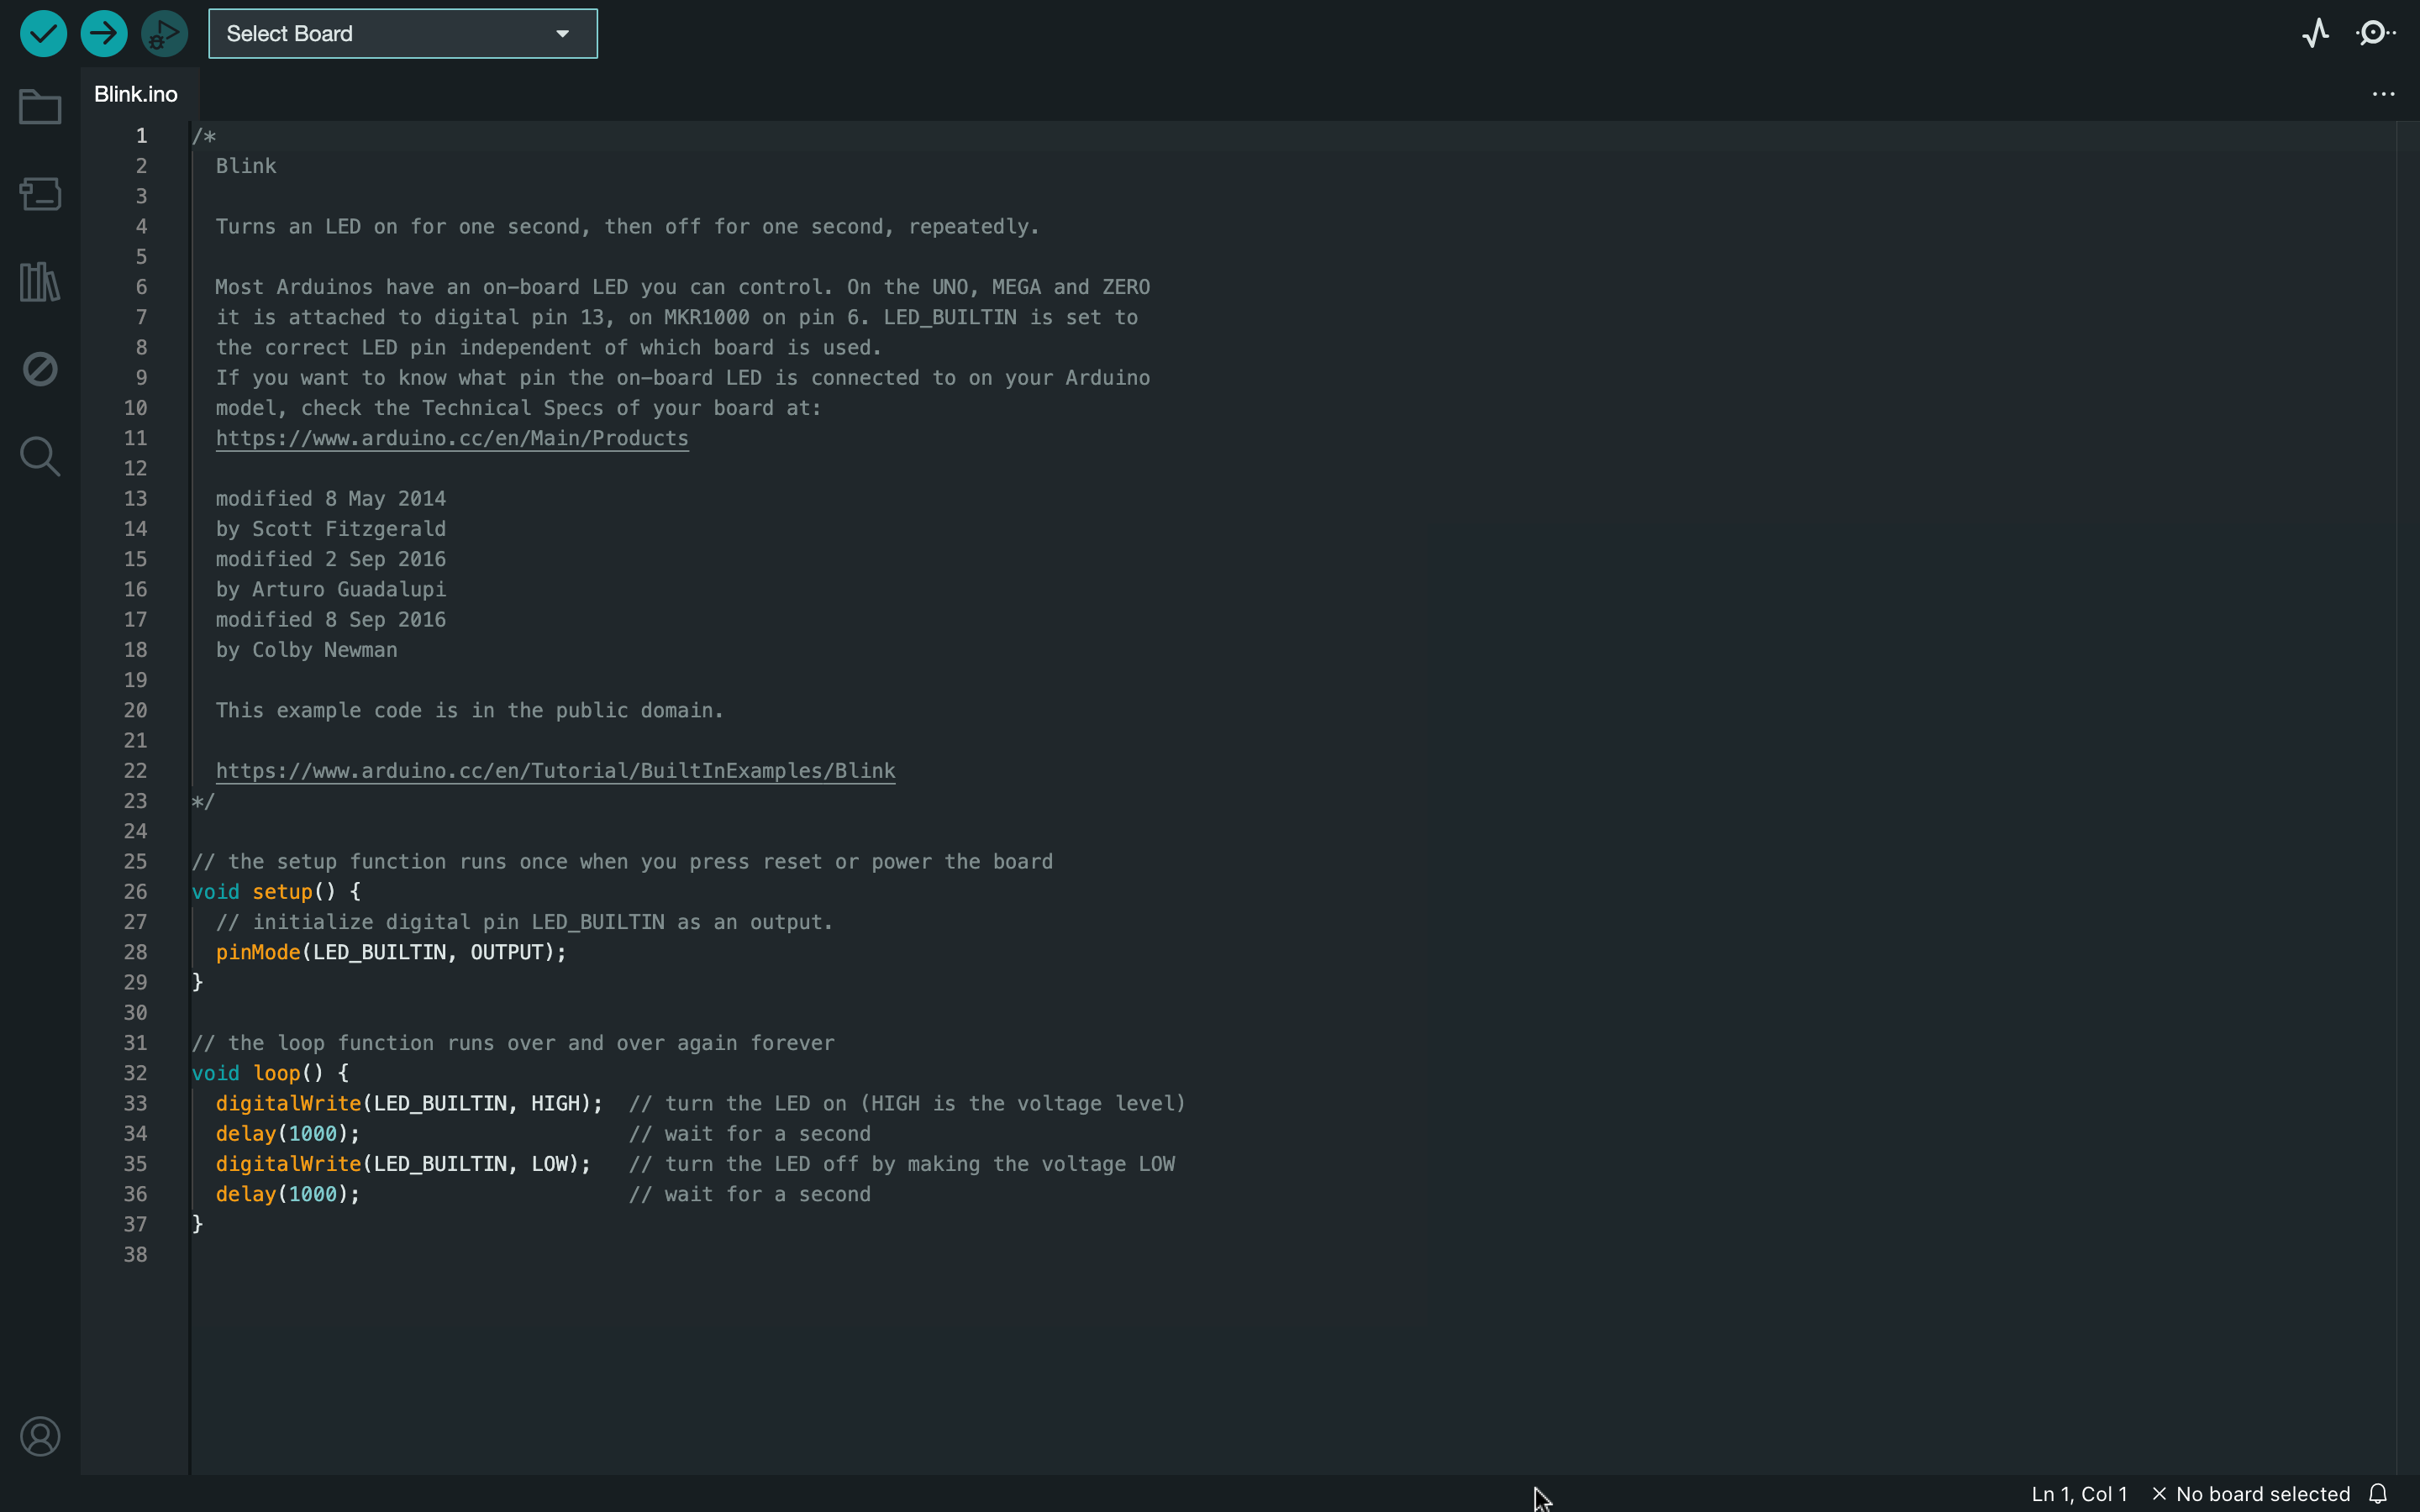
\includegraphics[width=0.7\linewidth]{images/ArduinoIDE/CompileBlinkSketch.png}
		\captionof{figure}{Blink Sketch Compile}
		\end{center}